%!TEX root = ../thesis_phd.tex
%%%%%%%%%%%%%%%%%%%%%%%%%%%%%%%%%%%%%%%%%%%%%%%%%%%%%%%%%%%%%%%%%%%%%%%%%%%%%%%%
%nuosc.tex: Chapter on neutrino physics:
%%%%%%%%%%%%%%%%%%%%%%%%%%%%%%%%%%%%%%%%%%%%%%%%%%%%%%%%%%%%%%%%%%%%%%%%%%%%%%%%
\chapter{Neutrino Physics}
\label{nu_osc_chapter}
%%%%%%%%%%%%%%%%%%%%%%%%%%%%%%%%%%%%%%%%%%%%%%%%%%%%%%%%%%%%%%%%%%%%%%%%%%%%%%%%

\section{Neutrino Interactions}

Neutrinos are neutral
\footnote{In the Standard Model, neutrality with regard to a force implies that
the particle does not couple to the force carriers of that force.}
to both the electromagnetic and strong forces.
Gravitational interactions are far too weak to observe.
Thus, the only neutrino interactions observed in practice are mediated
by the weak force \cite{halzen1984quarks}.

Weak interactions are mediated by either the \wb or \zb boson.
Diagrams depicting neutrino interactions can be seen in Figure \ref{nuInt}.
Since the \zb is neutral, the interactions it mediates are called
neutral current (NC) interactions, while those mediated by \wb are called
charged current (CC) interactions.
The distinction between NC and CC is an important one due to charge
conservation.
A particle interacting through a neutral boson is left with its charge
unchanged, while an interaction involving a charged boson must raise
or lower the charge of the interacting particle.
Thus, in an NC interaction, an interacting neutrino remains a neutrino.
CC interactions, on the other hand, will have an interacting neutrino converted
to its lepton partner.
To the observer, the outgoing lepton in a CC interaction serves as a signature
of the flavor of the interacting neutrino: for instance,
the presence of a muon implies that a muon neutrino interacted.
NC interactions, on the other hand, carry no flavor signature of the
interacting neutrino \cite{ho2010elementary}.

\begin{figure}
\begin{center}
  \begin{subfigure}[b]{0.45\textwidth}
    \centering
    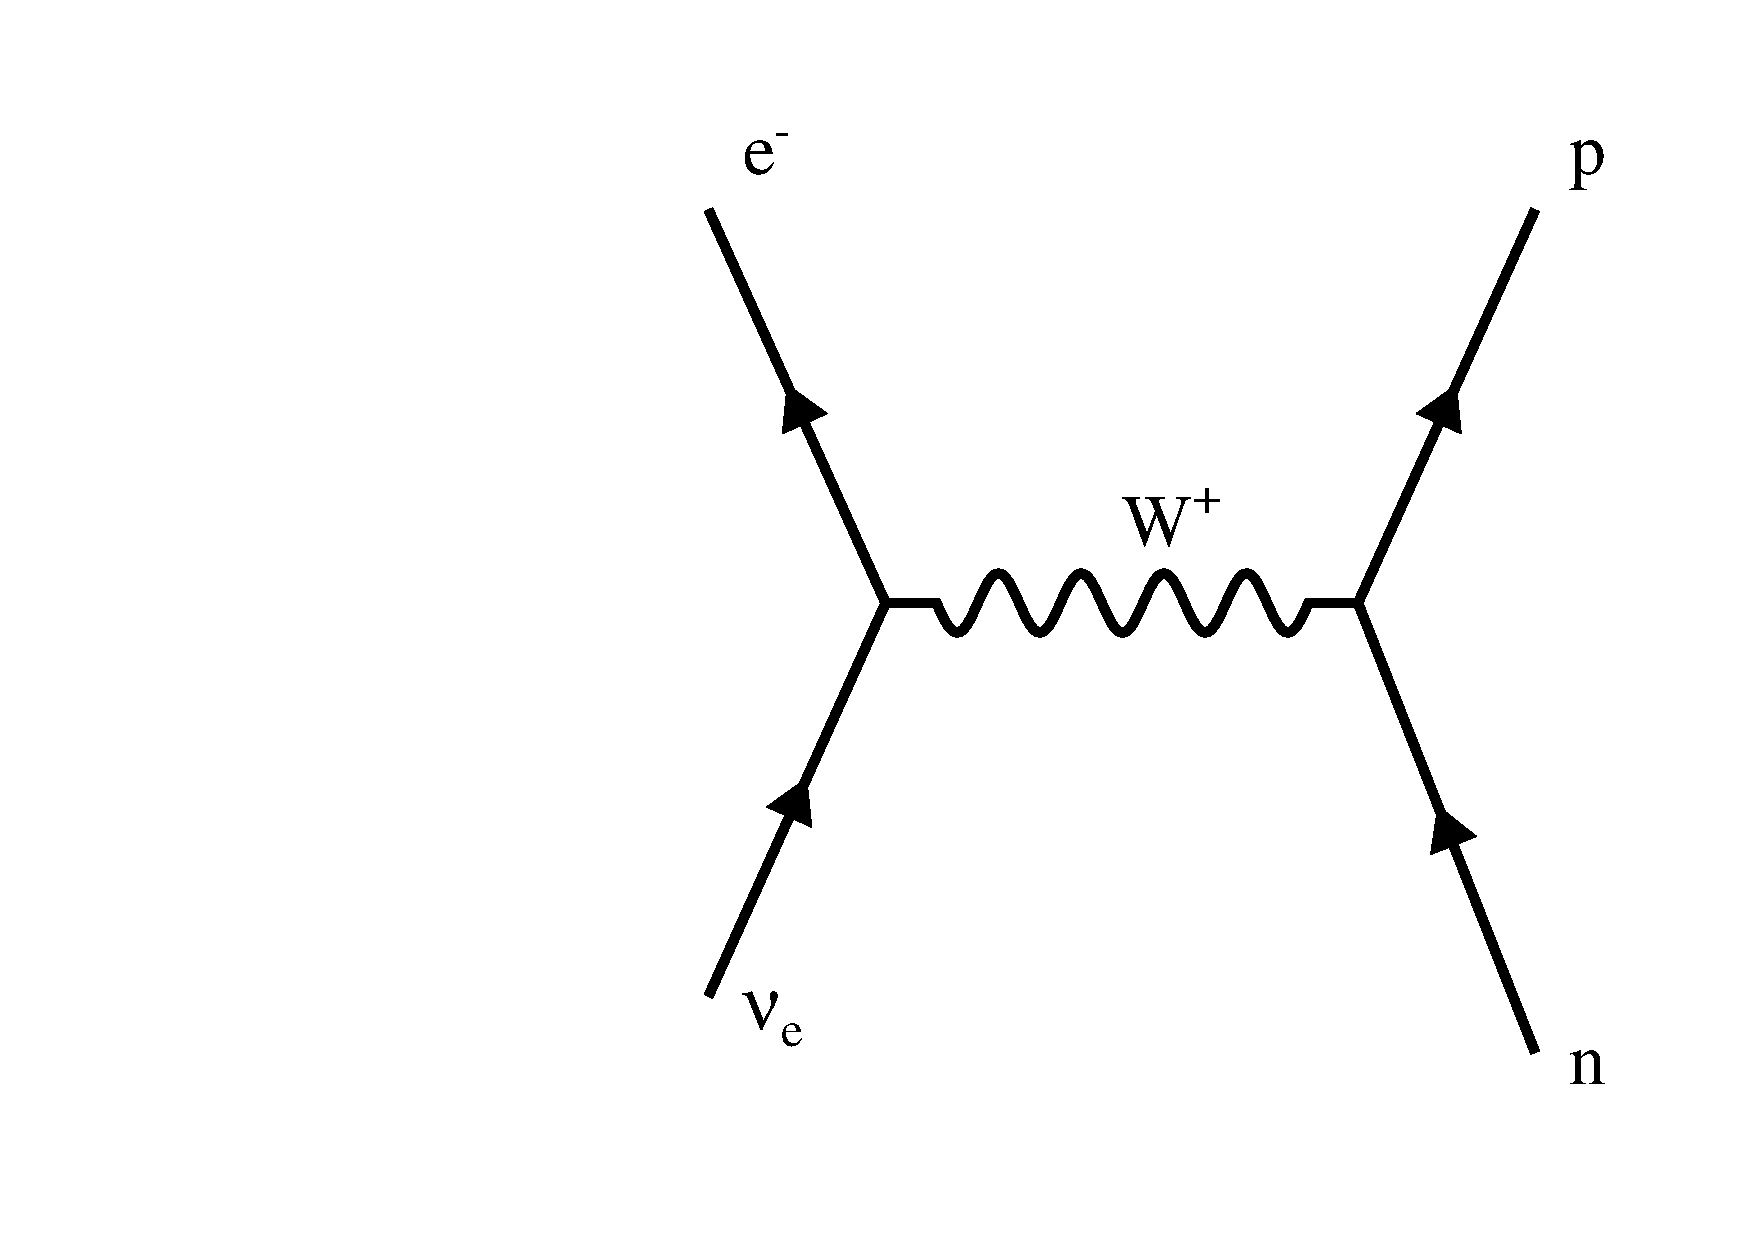
\includegraphics[width=\textwidth]{figures/feynman/ccNue.pdf}
    \caption*{$\nu_e + n \rightarrow e^- + p$}
     \label{ccNue}
  \end{subfigure}
  ~
  \begin{subfigure}[b]{0.45\textwidth}
    \centering
    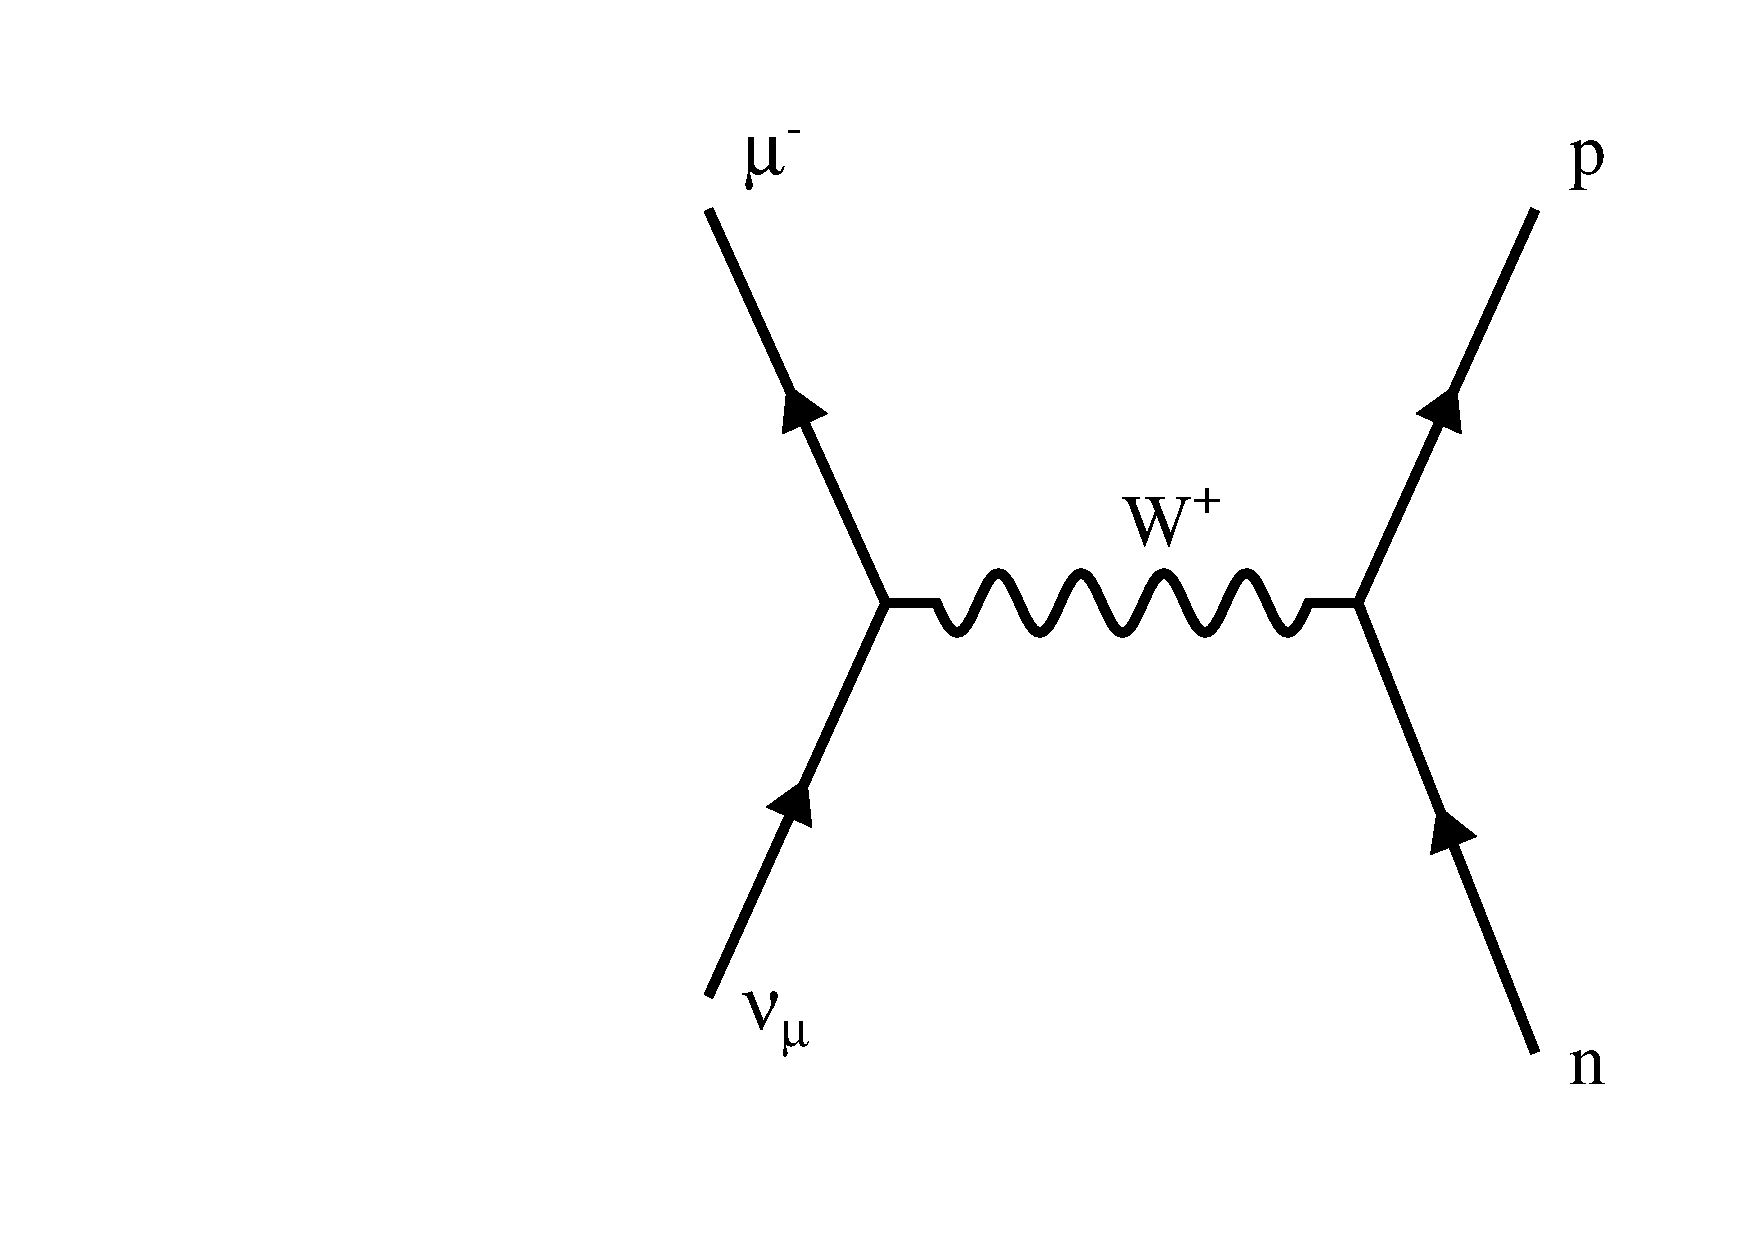
\includegraphics[width=\textwidth]{figures/feynman/ccNumu.pdf}
    \caption*{$\nu_\mu + n \rightarrow \mu^- + p$}
    \label{ccNumu}
  \end{subfigure}

  \vspace{20pt}
  \begin{subfigure}[b]{0.45\textwidth}
    \centering
    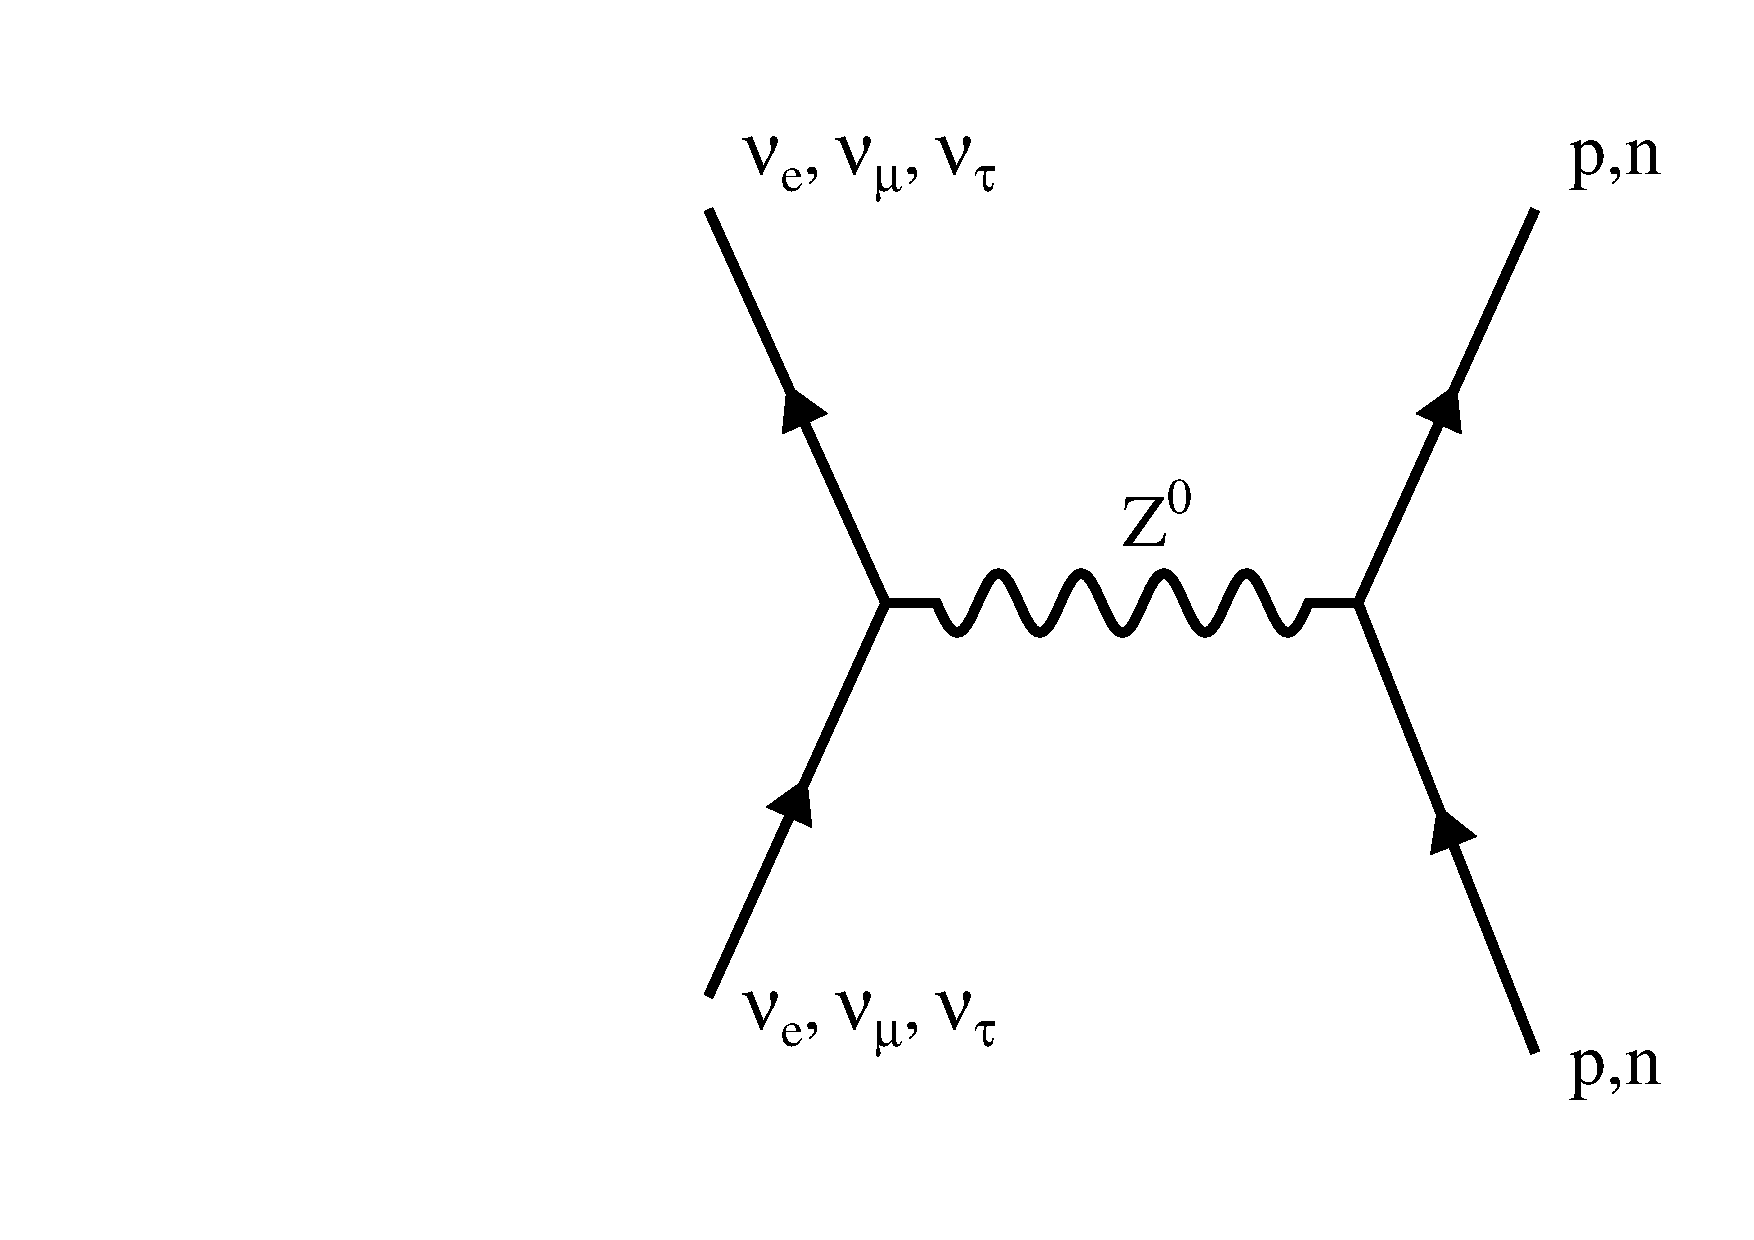
\includegraphics[width=\textwidth]{figures/feynman/ncHad.pdf}
    \caption*{$\nu + N \rightarrow \nu + N$}
  \end{subfigure}
  ~
  \begin{subfigure}[b]{0.45\textwidth}
    \centering
    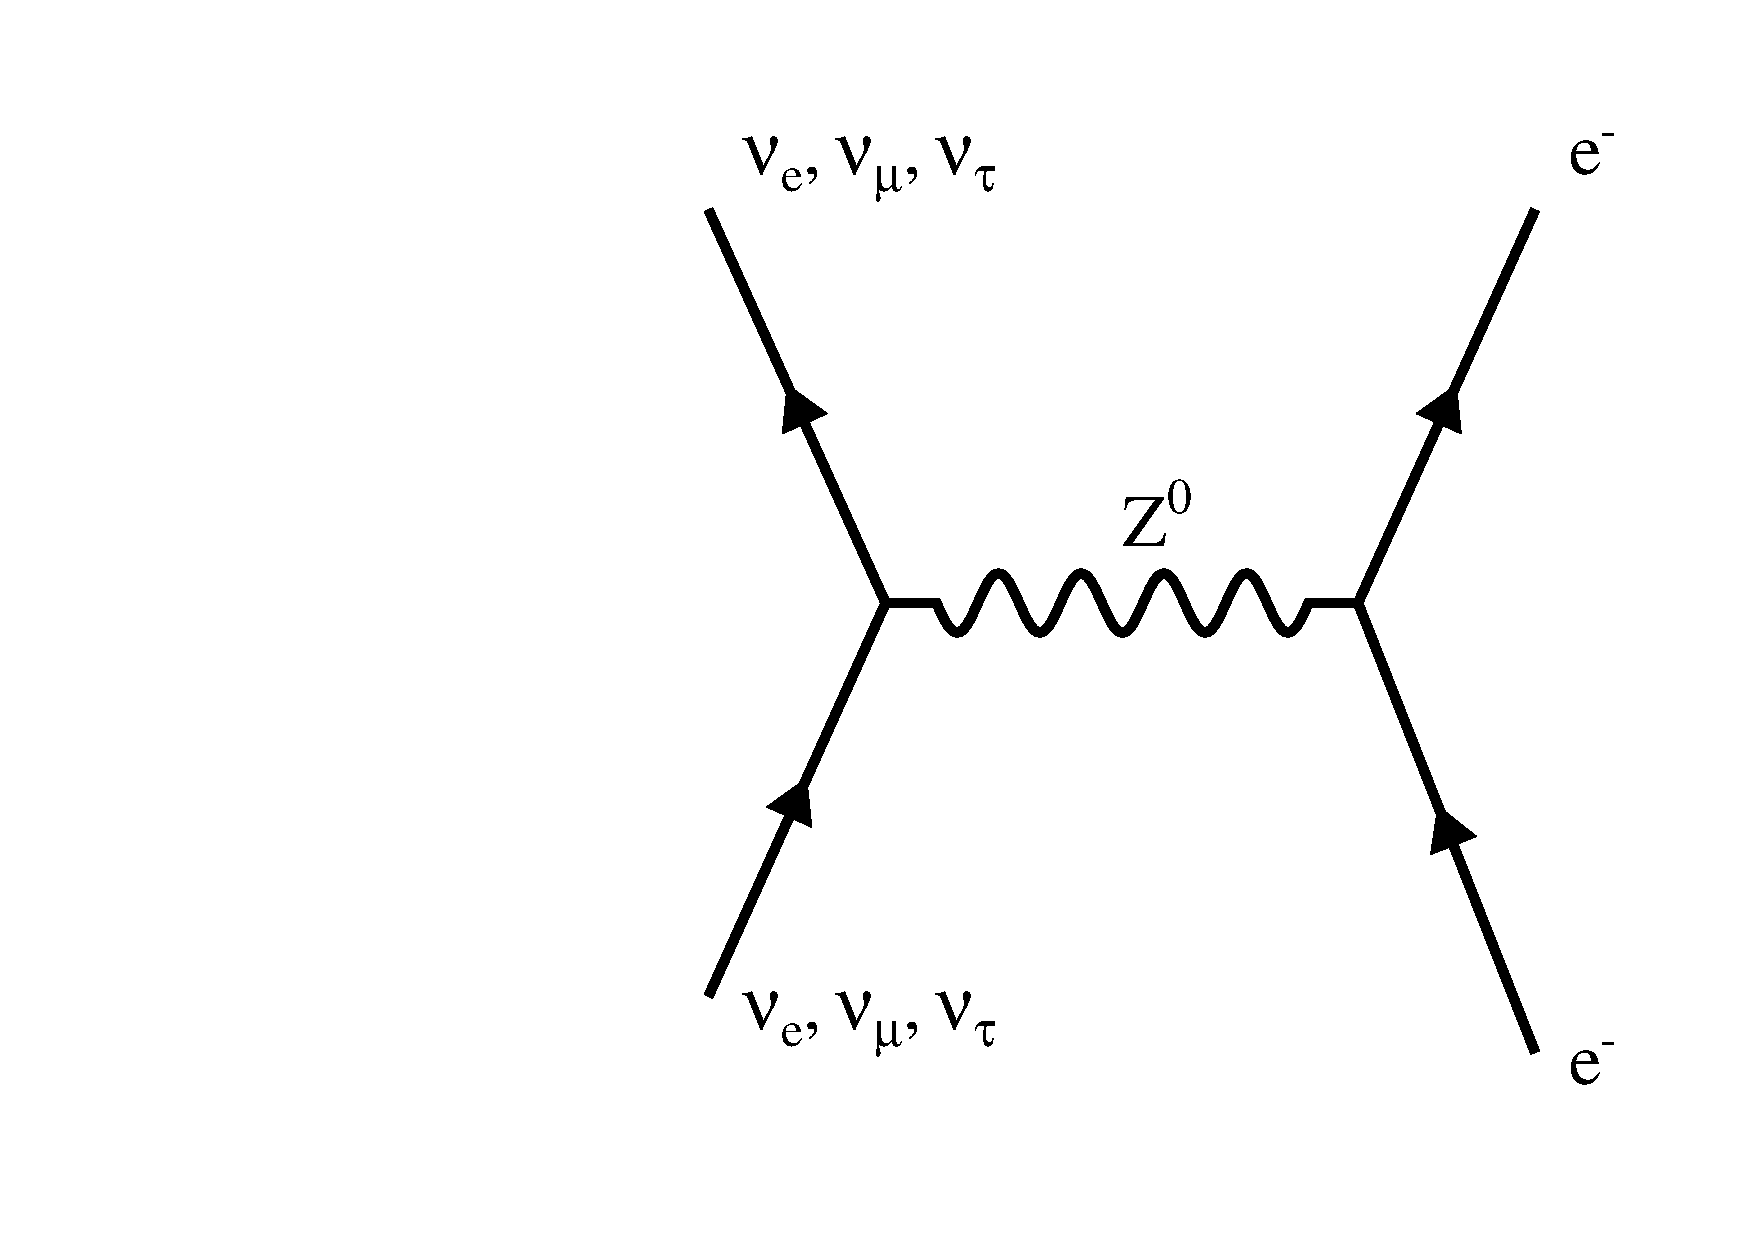
\includegraphics[width=\textwidth]{figures/feynman/ncElec.pdf}
    \caption*{$\nu + e^- \rightarrow \nu + e^-$}
  \end{subfigure}

\end{center}
\caption{Neutrino interaction diagrams}{
CC and NC interactions are mediated by \wb or \zb bosons, respectively.
All figures above are meant to be interpreted with the time axis running from
top to bottom, indicating a neutrino and some target exists
in the initial state.
The top panes show CC interactions, while the bottom panes show NC interactions.
The top left (right) pane shows an electron (a muon) neutrino interacting with
a neutron through a \wb
to produce an electron (a muon) and a proton in the final state.
The bottom left pane shows an NC interacting with nucleon, while
the bottom right pane shows an NC interaction with an electron.
Note that CC interactions with leptons, such as an electron, are permitted,
although they are far more rare.
An example of such an interaction can be seen in Figure \ref{ccElec}.
}
\label{nuInt}
\end{figure}

The vast majority of neutrino interactions observed in matter involve
scattering against a nuclear target.
Scattering with atomic electrons is permitted, although it happens at a
far lower rate due to the relatively small mass of the electron.
On the leptonic side of the scattering process, the incident neutrino
incident neutrino is either converted to a charged lepton in the CC case,
or remains a neutrino in the NC case.
The nuclear side of the interaction, however, can be far more messy
due to the structure of the nucleus.
The simplest case is called when the neutrino interacts with a
single nucleon without significant coupling to the nucleus.
For the NC case, this is called an elastic interaction
\cite{fuess1981neutrino}, while the CC version
is called a quasi-elastic (QE) interaction since the nucleon changes form
(e.g. neutron to proton) \cite{LlewellynSmith}.
A neutrino interaction can also excite a resonance within the nucleus to
produce a hadron, for instance, a pion;
these scattering events are referred to as resonant production
\cite{rein1981neutrino}.
More complicated scattering events which cause significant disturbance of the
nuclear system (and typically complete breakup) are called deep-inelastic
scattering (DIS) events \cite{lee1957parity,whitlow1990precise,aivazis1994leptoproduction}.


\section{Neutrino Oscillation}

\subsection{A Straightforward Interpretation}

Neutrinos are neutral to both the electromagnetic and strong forces.
The effects of gravity are too minute to observe at the energy scales
encountered in neutrino experiments.
Therefore, of the four fundamental forces,\footnote{All physical interactions
are thought to be mediated by one of four forces: the electromagnetic,
strong, weak and gravitational forces.} we only observe neutrinos interacting
through the weak force.
When a neutrino interacts, it does so in one of its three weak flavor states:
\nue, \numu or $\nu_\tau$.
But in contrast to our intuition, the flavor states do not have definite mass;
each is a mixture of three components with distinct masses: $\nu_1$, $\nu_2$
and $\nu_3$.
A neutrino produced in a particular flavor state--- for instance, an electron
neutrino produced in the sun--- is composed of some fraction of $\nu_1$, a
different fraction of $\nu_2$ and yet another fraction of $\nu_3$.
The mass components propagate as three distinct waves, summing together to make
a total wave that is the neutrino.
As these waves travel through space, they move in and out of phase with each
other to cause interference; as a result, the composition fractions of the
neutrino change.
For every composition of $\nu_1$, $\nu_2$ and $\nu_3$, there are distinct
probabilities of interacting as \nue, \numu or $\nu_\tau$.
Thus, when a neutrino reaches its interaction point--- say, the solar neutrino
arriving at Homestake mine--- its makeup will have changed to something that
may be more likely to interact as a different flavor.
The theory that describes this phenomenon is that of neutrino oscillation.

\subsection{Oscillation in Vacuum}

The weak flavor states are the eigenstates of the Hamiltonian of
weak interactions.
A neutrino produced as flavor $l = e, \mu, \tau$ can be written as a
superposition of mass states $\alpha = 1, 2, 3$ in terms of the elements of a
unitary $3\times3$ matrix $U_{l\alpha}$ as follows:
\begin{equation}\label{superpos}
|\nu_l \rangle = \sum_{\alpha = 1,}^3 U_{l\alpha}|\nu_\alpha \rangle
\end{equation} %check this, should it be U*?
This superposition describes a change of basis and can be likened to rotations
in a three dimensional space.
$U_{l\alpha}$ can be written in terms of three Euler angles --
\thetaot, \thetatth, and \thetaoth ~-- as well as a complex phase, $\delta$,
which allows for the possibility of CP violation
\footnote{CP (charge-parity) symmetry is a property which dictates a physical
process is invariant under inversion of charge and spatial orientation (parity).
A non-zero value of $\delta$ would indicate violation of CP symmetry\cite{ho2010elementary}.}.
The matrix $U_{l\alpha}$ (written here with $c_{ij}$ and $s_{ij}$ as shorthand
for
$\cos{\theta_{ij}}$ and $\sin{\theta_{ij}}$, respectively) is then the product
of the three rotations, commonly referred to as the
Pontecorvo-Maki-Nakagawa-Sakata (PMNS) matrix \cite{ho2010elementary}:
\begin{equation}
 U_{l\alpha} = \begin{pmatrix} \label{pmns}
c_{13}c_{12}              &    c_{13}s_{12}        &    s_{13} e^{-i\delta} \\
-s_{12}c_{23} - c_{12}s_{23}s_{13}e^{i\delta} & c_{12}c_{23} - s_{12}s_{23}s_{13}e^{i\delta}        &     c_{13}s_{23}  \\
s_{23}s_{12} - c_{12}c_{23}s_{13}e^{i\delta}  & -c_{12}s_{23} - s_{12}c_{23}s_{13}e^{i\delta}         &     c_{13}c_{23}  \\
\end{pmatrix}.
\end{equation}
This matrix, along with the superposition in \eqref{superpos} gives the
fractions of $\nu_1$, $\nu_2$ and $\nu_3$ that make up \nue, \numu or
$\nu_\tau$.
To see how neutrinos oscillate we must consider their time evolution:
\begin{equation}\label{evolve}
|\nu_l(t) \rangle = \sum_{\alpha = 1,}^3 U_{l\alpha}e^{-iE_\alpha t}|\nu_\alpha \rangle,
\end{equation}
where $E_\alpha$ represents the energy\footnote{Physical quantities are
displayed in natural units, $\hbar = c = 1$}
of the eigenstate, which depends on its mass and momentum:
\begin{equation}\label{energy}
E_\alpha = \sqrt{p_\alpha^2 + m_\alpha^2}
\end{equation}
For highly relativistic neutrinos, the momentum is much larger than the mass,
so we have
$|p_\alpha| \simeq |p| \simeq E$ allowing us to write \eqref{energy} as:
\begin{equation}\label{energyApprox}
E_\alpha \simeq p(1+\frac{m_\alpha^2}{2p^2})\simeq (E+\frac{m_\alpha^2}{2E}).
\end{equation}
We can then substitute this into \eqref{evolve}:
\begin{equation}\label{evolveSub}
|\nu_l(t) \rangle = e^{-iEt} \sum_{\alpha = 1,}^3 U_{l\alpha}e^{-i\frac{m_\alpha^2}{2E} t}|\nu_\alpha\rangle.
\end{equation}

To find the probability of observing the transition between flavor states
$\nu_l \rightarrow \nu_m$ (also valid for $l=m$, as in the case of
$\nu_\mu \rightarrow \nu_\mu$) we square the inner product between the two
states:
\begin{equation}\label{probSimp}
P_{l\rightarrow m}(t) = |\langle \nu_m | \nu_l(t)\rangle |^2.
\end{equation}
More explicitly, we have
\begin{equation}\label{probComp}
P_{l\rightarrow m}(t) = \sum_{\alpha = 1,}^3 \sum_{\beta = 1,}^3 U^*_{l\alpha}U_{m\alpha}U^*_{l\beta}U_{m\beta} e^{i\frac{m_\alpha^2}{2E}t} e^{-i\frac{m_\beta^2}{2E}t},
\end{equation}
which, through the unitarity of $U$ and use of some trigonometric identities,
can be written as:
\begin{equation}\begin{split}\label{oscProb}
P_{l\rightarrow m}(t) =  \delta_{lm} - 4  \sum_{\alpha > \beta}  \Re(U^*_{l\alpha}U_{m\alpha}U^*_{l\beta}U_{m\beta}) \sin^2 \bigg(\frac{\Delta m_{\alpha\beta}^2}{4E} t\bigg) \\
 + 2  \sum_{\alpha>\beta}  \Im(U^*_{l\alpha}U_{m\alpha}U^*_{l\beta}U_{m\beta}) \sin\bigg(\frac{\Delta m_{\alpha\beta}^2}{2E}t\bigg).
\end{split}\end{equation}
Here, $\delta_{lm}$ is the Kronecker delta and
$\Delta m^2_{\alpha\beta} = m_\alpha^2 - m_\beta^2$.
In equation~\eqref{oscProb}, the prefactors on the $\sin$ and $\sin^2$ terms
are real numbers that depend on the Euler angles \thetaot, \thetatth and
\thetaoth as well as the CP violating phase $\delta$.
For relativistic neutrinos, we can take $t \simeq L$, the distance between the
source and the interaction point; substituting this in \eqref{oscProb} yields a
form relevant for oscillation experiments:
\begin{equation}\begin{split}\label{oscProbL}
P_{l\rightarrow m}(L) =  \delta_{lm} - 4  \sum_{\alpha > \beta}  \Re(U^*_{l\alpha}U_{m\alpha}U^*_{l\beta}U_{m\beta}) \sin^2 \bigg(\frac{\Delta m_{\alpha\beta}^2}{4E} L\bigg) \\
 + 2  \sum_{\alpha>\beta}  \Im(U^*_{l\alpha}U_{m\alpha}U^*_{l\beta}U_{m\beta}) \sin\bigg(\frac{\Delta m_{\alpha\beta}^2}{2E}L\bigg).
\end{split}\end{equation}
It is interesting to note the dependence on the mass squared differences,
$\Delta m^2_{\alpha\beta}$ rather than the masses themselves.
As a result, oscillation experiments are not sensitive to absolute neutrino
masses.
Measurement of these parameters will be discussed in detail in later sections.

\subsection{Oscillation in Matter}\label{matOsc}
\label{osc_in_matter_section}

Neutrinos propagating in matter can scatter upon components of atoms through
the exchange of $W^\pm$ and $Z^0$ bosons.
In analogy to light propagating in matter, neutrinos can undergo coherent
scatterings with the surrounding particles.
Coherent scatterings are those which do not change the state of the system,
preserving the momentum and energy of the particles involved.

\begin{figure}
\begin{center}
\begin{subfigure}[b]{0.45\textwidth}
                \centering
                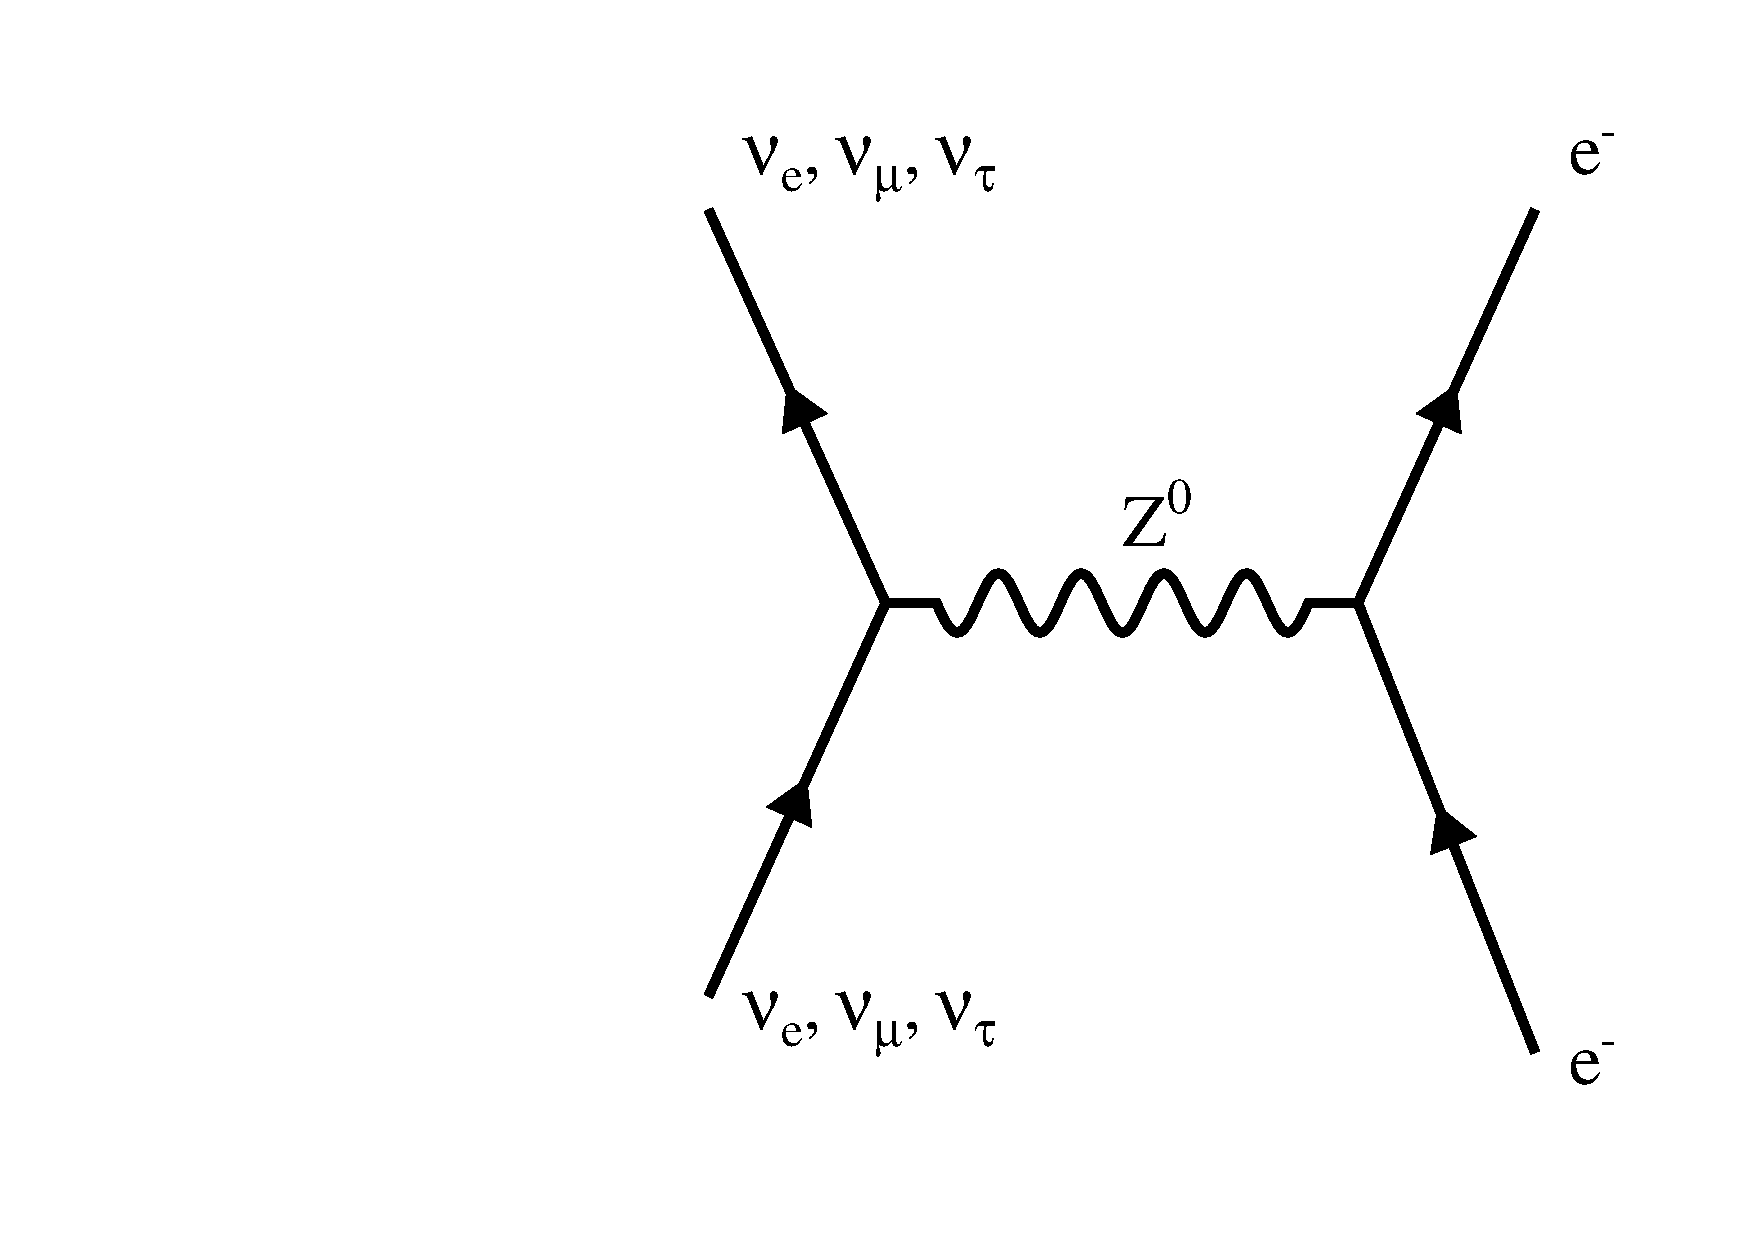
\includegraphics[width=\textwidth]{figures/feynman/ncElec.pdf}
                \caption{}
                 \label{ncElec}
        \end{subfigure}
        ~
\begin{subfigure}[b]{0.45\textwidth}
                \centering
                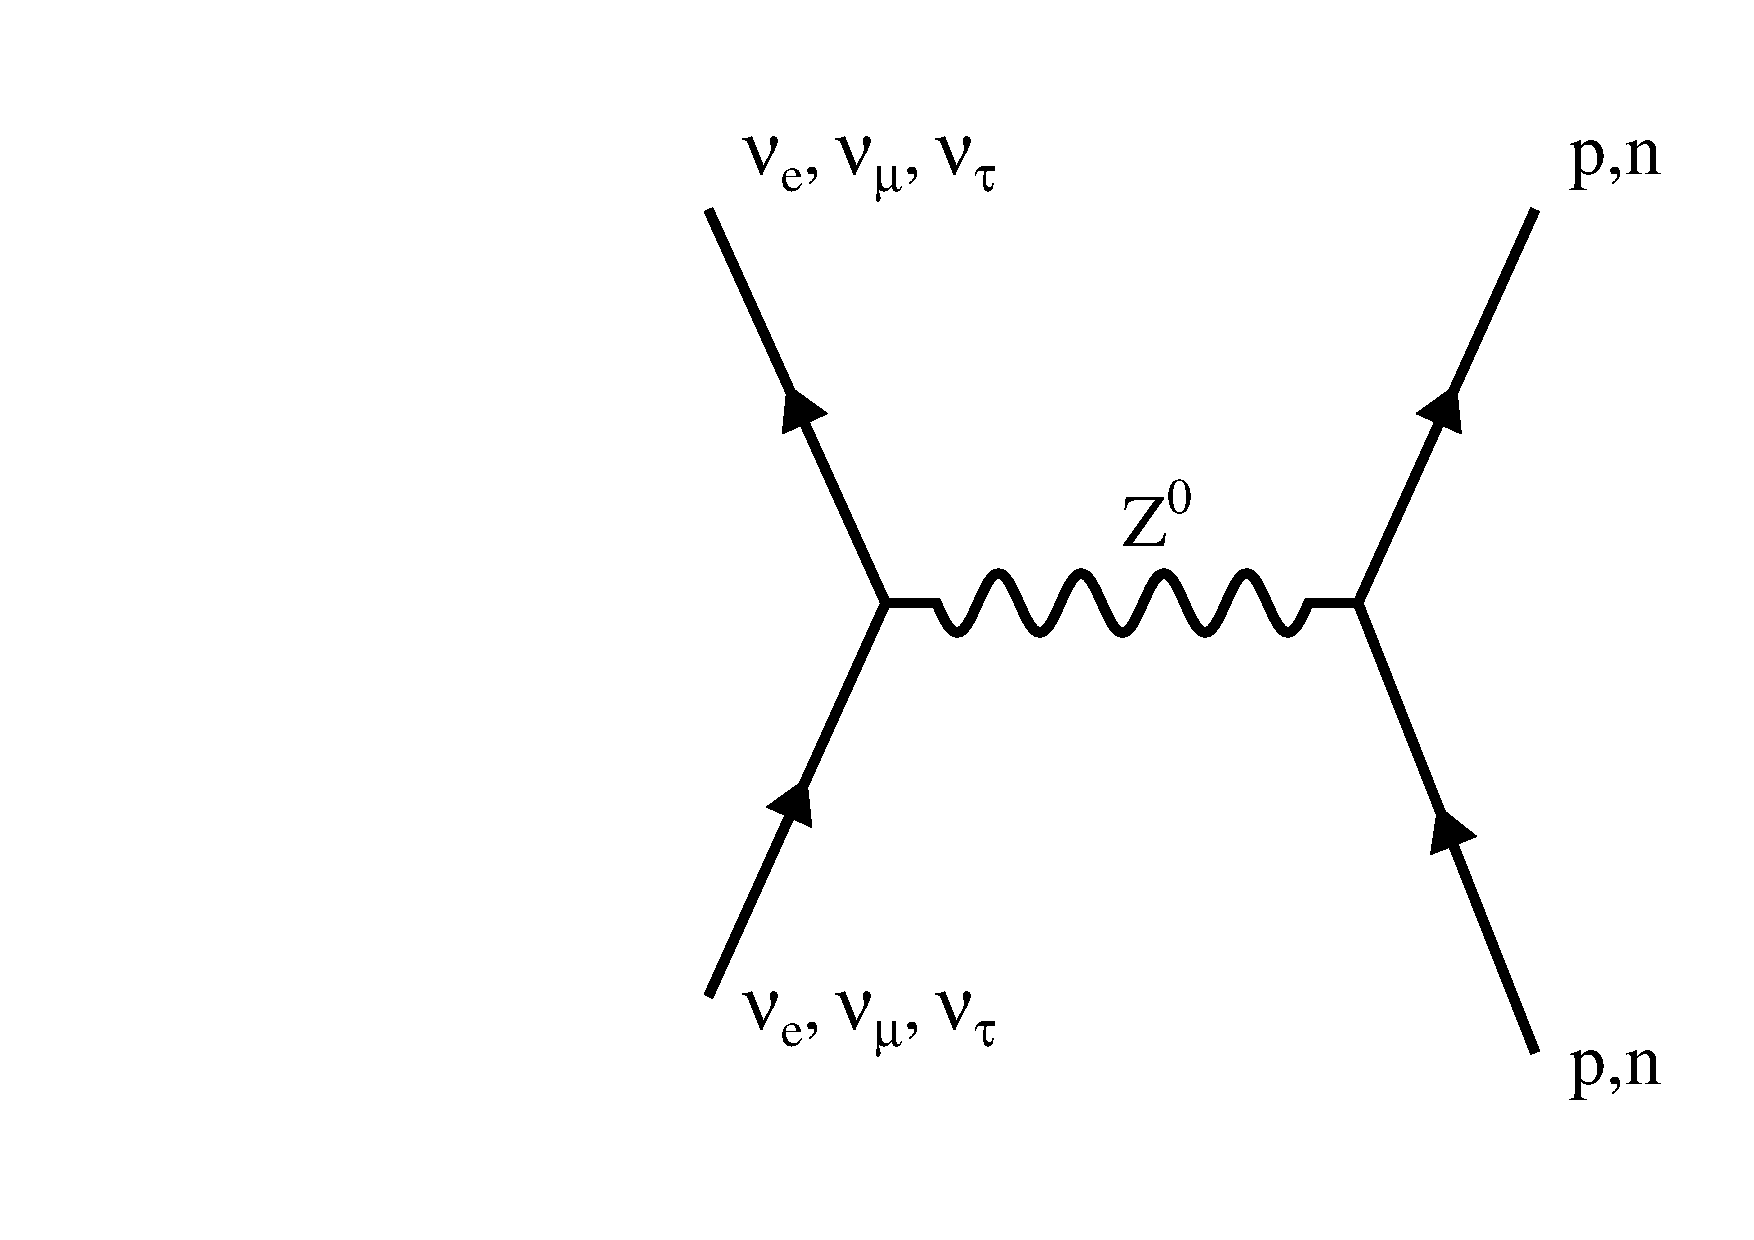
\includegraphics[width=\textwidth]{figures/feynman/ncHad.pdf}
                \caption{}
                 \label{ncHad}
        \end{subfigure}


        \begin{subfigure}[b]{0.45\textwidth}
                \centering
                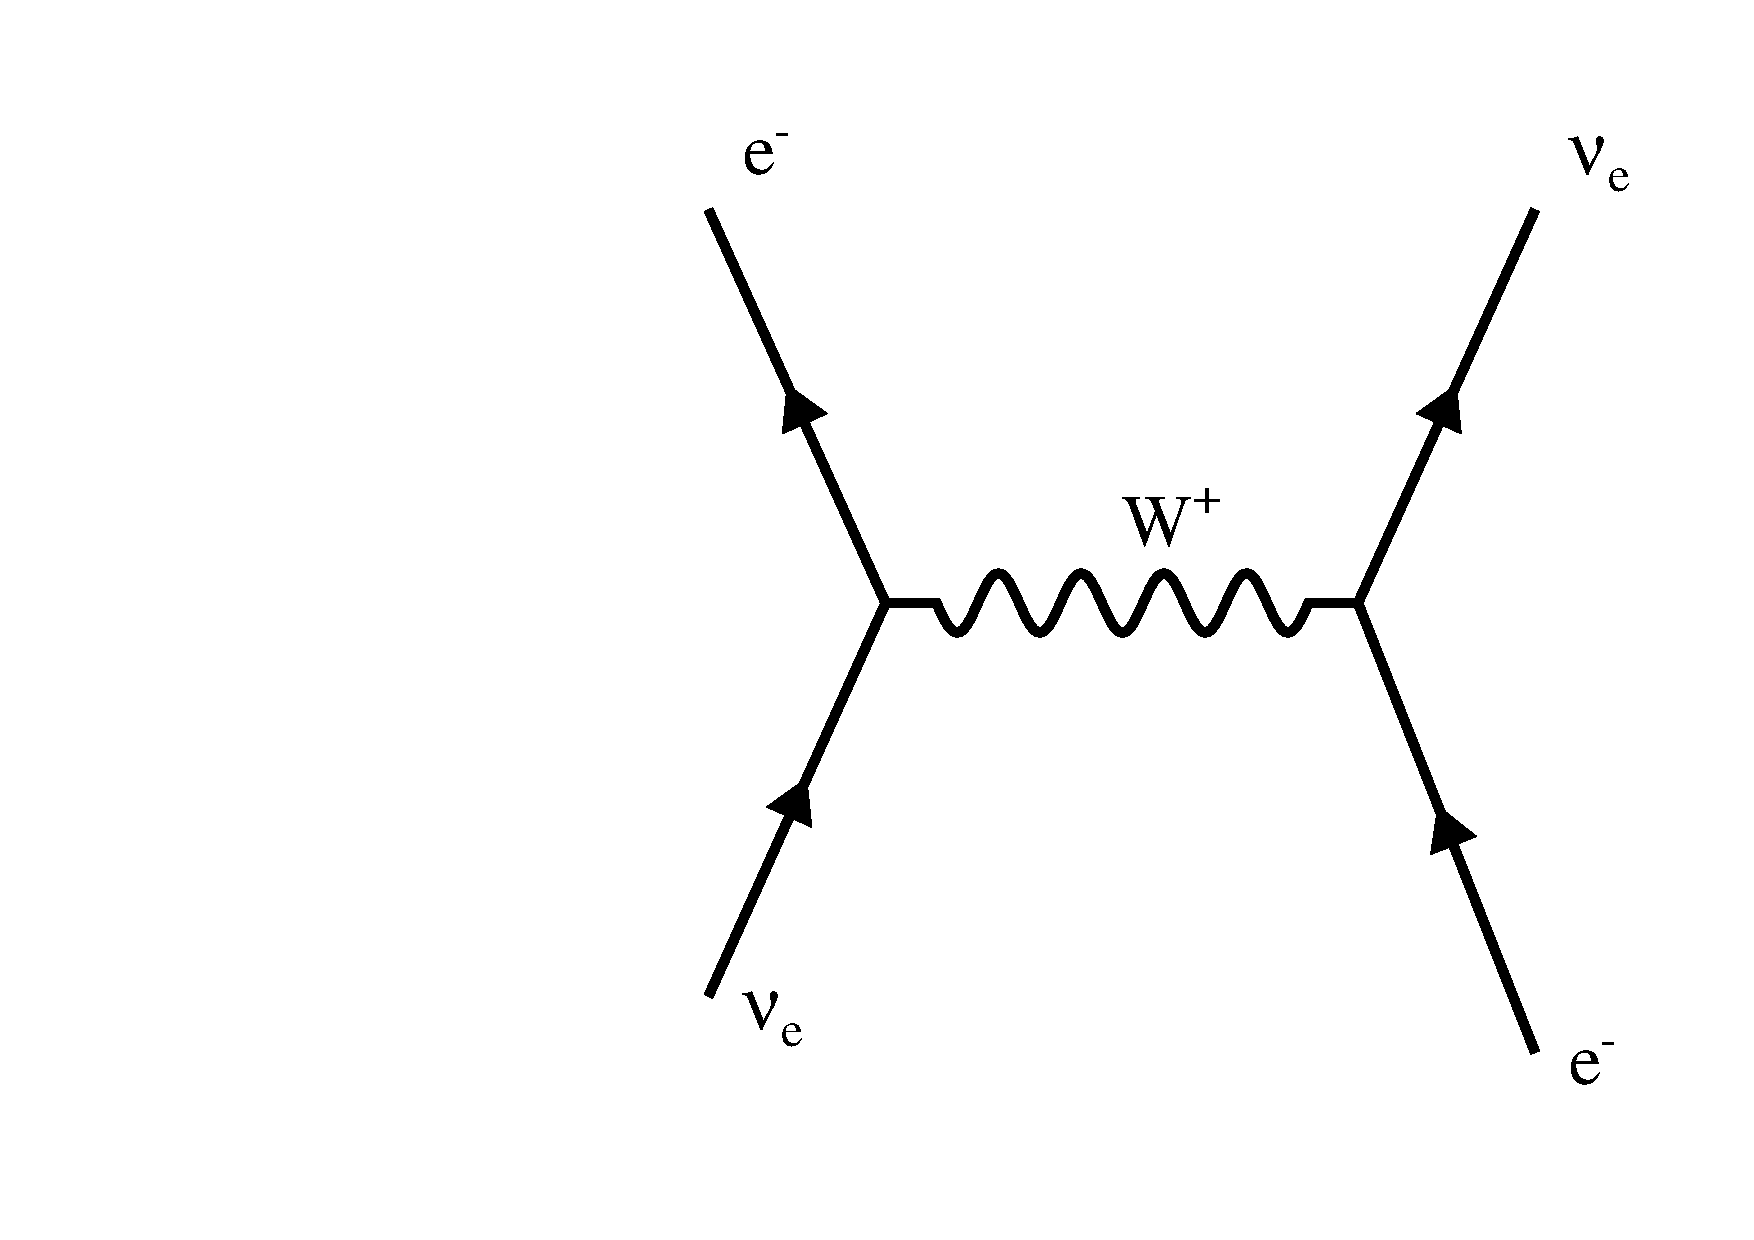
\includegraphics[width=\textwidth]{figures/feynman/ccElec.pdf}
                \caption{}
                 \label{ccElec}
        \end{subfigure}
\end{center}
\caption{Interactions that permit coherent scattering.}{
Coherent interactions are those which leave the momentum
and flavor of the scattering products unchanged.
In all three diagrams, the time axis runs from bottom to top.
The top left pane shows NC neutrino scattering electron scattering against an
atomic electron, whereas the top right shows scattering with an atomic
nucleon.
The bottom shows a CC scattering with an atomic electron;
while the electron and \nue have switched positions, the initial and
final state are identical.
}
\label{cohScatter}
\end{figure}
A quantitative treatment of this phenomenon imparts particles with an effective
mass that modifies their physical mass.
In the case of light, the effective mass manifests itself in the familiar index
of refraction that diminishes the speed of light in matter.
For neutrinos, coherent scattering interactions are mediated through the
exchange of $W^\pm$ and $Z^0$ bosons; the Feynman diagrams for these
interactions can be seen in Figure~\ref{cohScatter}.
The neutral current interactions (those moderated by $Z^0$ exchange) are the
same for all three neutrino flavors and have no effect on oscillation
probabilities.
On the other hand, since terrestrial matter contains electrons but not muons
and taus, the charged-current interaction with electrons only occurs for \nue,
giving rise to an effective potential \cite{ho2010elementary}:
\begin{equation}
\label{veff}
V_{CC} = \sqrt{2}G_F n_e,
\end{equation}
where $n_e$ is the number density of electrons in the medium and $G_F$ is
Fermi's constant.
Since this effective potential only exists for electrons, it modifies the
oscillation probabilities given in equation \eqref{oscProbL}, specifically
changing the sine term \cite{ho2010elementary}:
\begin{equation}
\label{modSin}
\sin\bigg(\frac{\Delta m_{\alpha\beta}^2}{2E}L\bigg) \rightarrow
\frac{\Delta m_{\alpha\beta}^2}{\Delta m_{\alpha\beta}^2 \pm E V_{CC}/2} \sin\bigg((\frac{\Delta m_{\alpha\beta}^2}{2E} \pm \frac{EV_{CC}}{2})L \bigg).
\end{equation}
with the $\pm$ corresponding to a difference in sign for neutrinos and
antineutrinos, respectively.
This effect is known as the Mikheyev-Smirnov-Wolfenstein (MSW) effect
\cite{wolfenstein1978neutrino}.

\subsection{Recent Experiments and Results}
In the last two decades experimental neutrino physics has turned the corner
from an era of discovery to an era of precision.
The field has made this transition through the use of plentiful sources of
neutrinos as well as the development of kiloton scale detectors.
Interestingly enough, despite the growth in scale of neutrino experiments, the
techniques have remained largely the same as those of the discovery era.

Reactor neutrino experiments \cite{kamland, dayaBay, reno} have become
sensitive enough to measure the survival probability for electron
antineutrinos, $P(\bar{\nu_e} \rightarrow \bar{\nu_e})$.
Accelerator neutrino experiments \cite{minos13,abe2014observation,nova2016nue}
can now
measure similar probabilities for muon neutrinos, namely,
$P(\nu_\mu \rightarrow \nu_\mu$) and $P(\nu_\mu \rightarrow \nu_e)$.
In addition to these common sources, a third plentiful source comes in the form
of atmospheric neutrinos.
Cosmic-ray protons interacting in the upper atmosphere produce showers of
predominantly pions and kaons that then decay into neutrinos.
If a detector can reconstruct the zenith angle of an atmospheric neutrino, it
can determine the distance between its creation and interaction points.
Therefore, a detector that can sample all zenith angles in turn samples a wide
range of neutrino baselines ranging from the height of the atmosphere up to the
diameter of the earth.

The mixing angles have now all been measured to be nonzero by measuring either
survival or appearance probabilities.
Precise measurements of \thetaot, the ``solar" mixing angle, have been
performed by solar neutrino experiments such as SNO and reactor experiments
such as KamLAND \cite{sno, kamland, pdg}.
 These measurements yield $\theta_{12} \approx 34^\circ$ with about one
 $1^\circ$ of uncertainty.
The ``atmospheric" mixing angle, \thetatth has been measured as
$\sin^2(\theta_{23}) =  0.514^{+0.055}_{-0.056}$ by neutrino observatories
such as SNO and Super-Kamiokande (Super-K) as well as long baseline
experiments such as MINOS \cite{sno, superK, minos, pdg}.
Most recently, Daya Bay, RENO, MINOS, T2K, and \nova have made measurements of
\thetaoth that are not consistent with zero
\cite{dayaBay, reno, minos13,abe2014observation}.
The PDG best fit gives $\sin^2(2 \theta_{13}) \approx 0.085 \pm 0.005$

Measurements have also been made of the squared-mass differences.
It is known that $\Delta m_{21}^2$ is $(7.53 \pm 0.18) \times 10^{-5}$ eV${}^2$
and that $|\Delta m_{32}^2|$ is much larger at $(2.42 \pm 0.06) \times10^{-3}$
eV${^2}$.
This means that $\nu_1$ and $\nu_2$ could be similar in mass and that $\nu_3$
is relatively disparate in mass.
A remaining question is the sign of \deltamtht, commonly called the ordering of
the mass hierarchy.
In other words, we do not know whether $\nu_3$ is heavier (referred to as a
normal hierarchy) or considerably lighter (inverted hierarchy) than its
counterparts.

The work presented here will make measurements of $\sin^2(\theta_{23})$ and
\deltamtht.


%%%%%%%%%%%%%%%%%%%%%%%%%%%%%%%%%%%%%%%%%%%%%%%%%%%%%%%%%%%%%%%%%%%%%%%%%%%%%%%%
